% Exam Template for UMTYMP and Math Department courses
%
% Using Philip Hirschhorn's exam.cls: http://www-math.mit.edu/~psh/#ExamCls
%
% run pdflatex on a finished exam at least three times to do the grading table on front page.
%
%%%%%%%%%%%%%%%%%%%%%%%%%%%%%%%%%%%%%%%%%%%%%%%%%%%%%%%%%%%%%%%%%%%%%%%%%%%%%%%%%%%%%%%%%%%%%%

% These lines can probably stay unchanged, although you can remove the last
% two packages if you're not making pictures with tikz.
\documentclass[11pt]{exam}
\RequirePackage{amssymb, amsfonts, amsmath, latexsym, verbatim, xspace, setspace}
\RequirePackage{tikz, pgflibraryplotmarks}

% By default LaTeX uses large margins.  This doesn't work well on exams; problems
% end up in the "middle" of the page, reducing the amount of space for students
% to work on them.
\usepackage[margin=1in]{geometry}

\usetikzlibrary{calc}
\usepackage{graphicx}

% Here's where you edit the Class, Exam, Date, etc.
\newcommand{\class}{Initiation \`a l'algorithmique}
\newcommand{\term}{X2I0040, groupe 211}
\newcommand{\examnum}{CC 1}
\newcommand{\examdate}{27/03/2017}
\newcommand{\timelimit}{60 Minutes}

\usepackage{fancyvrb}
\fvset{frame=single,framesep=1mm,fontfamily=courier,fontsize=\normalsize,numbers=left,framerule=.3mm,numbersep=1mm,commandchars=\\\{\}}
\definecolor{dgreen}{rgb}{0.0, 0.5, 0.0}
\definecolor{ballblue}{rgb}{0.13, 0.67, 0.8}

\usepackage[absolute,overlay]{textpos}
\usepackage{caption}

% For an exam, single spacing is most appropriate
\singlespacing
% \onehalfspacing
% \doublespacing

% For an exam, we generally want to turn off paragraph indentation
\parindent 0ex

\begin{document} 

\begin{tikzpicture}[overlay, remember picture]
\node[anchor=north west, %anchor is upper left corner of the graphic
      xshift=2.5cm, %shifting around
      yshift=-0.8cm] 
     at (current page.north west) %left upper corner of the page
     {
\includegraphics[width=16.4cm]{UN_logo.png}}; 
\end{tikzpicture}

% These commands set up the running header on the top of the exam pages
\pagestyle{head}
\firstpageheader{}{}{}
\runningheader{\class}{\examnum\ - Page \thepage\ of \numpages}{\examdate}
\runningheadrule

\begin{flushright}
\begin{tabular}{p{2.8in} r l}
\textbf{\class} && \\%\makebox[2in]{\hrulefill}\\
\textbf{\term} &&\\
\textbf{\examnum} &&\\
\textbf{\examdate} &&\\
\textbf{Dur\'{e}e: \timelimit} & \textbf{Nom, Pr\'enom:} & \makebox[2in]{\hrulefill}
\end{tabular}\\
\end{flushright}
\rule[1ex]{\textwidth}{.1pt}

\noindent\fbox{%
\parbox{0.98\textwidth}{%
\textbf{Pr\'eambule} : Aucun document autoris\'e. Calculatrices et t\'el\'ephones portables interdits. Les exercices ne sont pas class\'es par difficult\'e croissante. 
Nombre de pages : \numpages
}%
}
\vspace{12pt}

%\begin{minipage}[t]{3.7in}
%\vspace{0pt}
%\begin{itemize}
%
%\item \textbf{If you use a ``fundamental theorem'' you must indicate this} and explain
%why the theorem may be applied.
%
%\item \textbf{Organize your work}, in a reasonably neat and coherent way, in
%the space provided. Work scattered all over the page without a clear ordering will 
%receive very little credit.  
%
%\item \textbf{Mysterious or unsupported answers will not receive full
%credit}.  A correct answer, unsupported by calculations, explanation,
%or algebraic work will receive no credit; an incorrect answer supported
%by substantially correct calculations and explanations might still receive
%partial credit.
%
%
%\item If you need more space, use the back of the pages; clearly indicate when you have done this.
%\end{itemize}
%
%Do not write in the table to the right.
%\end{minipage}
%\hfill
%\begin{minipage}[t]{2.3in}
%\vspace{0pt}
%%\cellwidth{3em}
%\gradetablestretch{2}
%\vqword{Problem}
%\addpoints % required here by exam.cls, even though questions haven't started yet.	
%\gradetable[v]%[pages]  % Use [pages] to have grading table by page instead of question
%
%\end{minipage}
%	\newpage % End of cover page

%%%%%%%%%%%%%%%%%%%%%%%%%%%%%%%%%%%%%%%%%%%%%%%%%%%%%%%%%%%%%%%%%%%%%%%%%%%%%%%%%%%%%
%
% See http://www-math.mit.edu/~psh/#ExamCls for full documentation, but the questions
% below give an idea of how to write questions [with parts] and have the points
% tracked automatically on the cover page.
%
%
%%%%%%%%%%%%%%%%%%%%%%%%%%%%%%%%%%%%%%%%%%%%%%%%%%%%%%%%%%%%%%%%%%%%%%%%%%%%%%%%%%%%%

\begin{questions}

% Basic question
%\addpoints
\question Pour v\'erifier qu'un nombre $N$ est \textbf{binaire}, on le divise successivement $p$ fois pas 10 (o\`u $p$ est le nombre de chiffres composant $N$ moins un), en v\'erifiant \`a chaque division que le reste appartiennent \`a l'ensemble $\{0,1\}$.

Par exemple, pour v\'erifier que le nombre $N = 101$ est un nombre \textbf{binaire}, on proc\`ede comme suit :

\begin{Verbatim}
n <- 101
r <- n {\bf mod} 10 = 1
r = 1 \textcolor{dgreen}{est dans} \{0,1\} \textcolor{dgreen}{alors... OK !}
n <- n {\bf div} 10 = 10
r <- n {\bf mod} 10 = 0
r = 0 \textcolor{dgreen}{est dans} \{0,1\} \textcolor{dgreen}{alors... OK !}
n <- n {\bf div} 10 = 1
r <- n {\bf mod} 10 = 1
r = 1 \textcolor{dgreen}{est dans} \{0,1\} \textcolor{dgreen}{alors... OK !}
\textcolor{dgreen}{Toutes les restes appartenaient \`a l'ensemble \{0,1\}, donc : }
	\textcolor{dgreen}{\bf N est BINAIRE}
\end{Verbatim}

Si dans l'une des \'etapes num\'ero 3, 6, ou 9, le reste \texttt{r} n'appartient pas \`a l'ensemble $\{0,1\}$, alors l'algorithme termine en affichant que le nombre $N$ n'est pas \textbf{binaire}.

\underline{\bf Question 1} Traduisez l'algorithme pr\'ec\'edent en code {\sc AlgoScript}.

\underline{\bf Question 2 (bonus)} \'Ecrivez un algorithme pour convertir n'importe quel nombre entier en \textbf{binaire}.

\question \'Etant donn\'e un tableau \textbf{T} d'entiers, \'ecrire une fonction \textcolor{ballblue}{\bf occurrences} qui retourne la quantit\'e de fois qu'un \'el\'ement $e$ est pressent dans ce tableau.

\underline{Exemple : } Si $T = [3, 6, 3, 8, 5, 3, 9, 7, 4, 5, 3]$, l'\'el\'ement $e = 3$ se trouve \textbf{4} fois dans le tableau.

% Question with parts
\newpage
%\addpoints
\question On suppose disposer de la fonction :

\begin{Verbatim}
\textcolor{blue}{\bf fonction} \textcolor{ballblue}{\bf etoile}(nomb : \textcolor{dgreen}{entier}) : \textcolor{dgreen}{chaine}
{\bf Variables}
	etoiles : \textcolor{dgreen}{chaine}
	i : \textcolor{dgreen}{entier}
{\bf Debut}
	etoiles <- ""
	\textcolor{blue}{\bf pour} i \textcolor{blue}{\bf allant de} 1 \textcolor{blue}{\bf a} nomb \textcolor{blue}{\bf faire} 
		etoiles <- etoiles + "*"; 
	\textcolor{blue}{\bf fin pour}
	\textcolor{blue}{\bf retourner} (etoiles) 
{\bf Fin}
\end{Verbatim}

En utilisant la fonction \textcolor{ballblue}{\bf etoile}, \'ecrire un algorithme affichant le texte suivant :

\begin{figure}[h!]
\centering
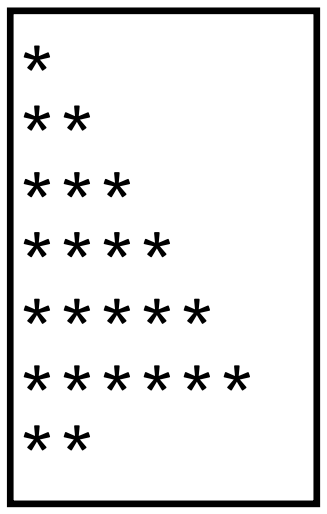
\includegraphics[height=5cm]{out1.png}
\captionsetup{labelformat=empty}
%\caption{Une figure.}
\end{figure}

%\begin{parts}
%\part[5] Find $f'(x)$ using the limit definition of derivative.
%\vfill
%\part[5] Find the line tangent to the graph of $y=f(x)$ at the point where $x=2$.
%\vfill
%\end{parts}

% If you want the total number of points for a question displayed at the top,
% as well as the number of points for each part, then you must turn off the point-counter
% or they will be double counted.
%\newpage
%\addpoints

\question (\textbf{bonus}) Le jeu de \textit{chasseur-proie} en une dimension consiste \`a faire partir un chasseur d'une position (g\'en\'eralement \`a la position 0) d'un tableau, et le faire chasser une proie situ\'ee sur une autre position du tableau. Si le chasseur marche avec une vitesse (quantit\'e de cases qu'il peut parcourir \`a chaque fois) \'egal \`a un, une proie situ\'ee \`a la position $k$ sera \'elimin\'ee en $k$ pas. Maintenant, consid\'erons que ce pas soit une quantit\'e donn\'ee.

Quand le chasseur d\'epasse la derni\`ere case du tableau, il recommence au d\'ebut (case 0) et compl\`ete son avancement. 

\underline{\bf Exemple : }

\begin{figure}[h!]
\centering
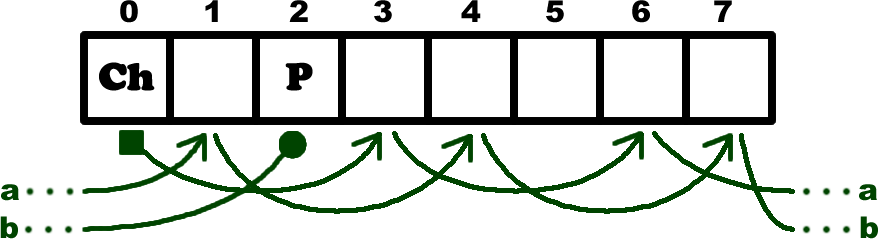
\includegraphics[height=2cm]{chP.png}
\captionsetup{labelformat=empty}
%\caption{Une figure.}
\end{figure}

Dans cet exemple, avec un pas \'egal \`a trois, un chasseur a besoin de six mouvements pour chasser la proie : $(3, 6, 1, 4, 7, 2)$.

On doit aussi analyser le cas o\`u le chasseur ne peut jamais chasser la proie.

\underline{\bf Question 1} \'Ecrivez une fonction qui re\c coit trois nombres entiers (la taille du tableau, la position de la proie et la vitesse du chasseur) et qui retourne la quantit\'e de mouvements dont le chasseur \`a besoin pour chasser la proie.
\end{questions}
\end{document}